\section{Ancient to Modern Mathematics: Fourier Analysis}

Joseph Fourier (1768-1830) was a . Fourier stated that any function can be represented by an infinite sum of sinusoids.

Through Euler's formula, this also means that any complex valued function can be written as the sum of complex exponentials.
 $$z(t)=\sum_{n=-\infty}^{\infty} a_n e^{int}$$
 
 If we expand out this infinite series, it would look something like

 $$ z(t) = \ldots a_{-2}e^{-2it} +  a_{-1}e^{-1it} + a_{0} + a_{1}e^{1it} + a_{2}e^{2it} + \ldots a_{k}e^{kit} + \ldots $$ 
 


Suppose that we are interested in deriving an explicit formula for some coefficient $a_k$. We must first isolate it by removing its other term $e^{ikt}$. This can be done by multiplying the entire series by $e^{-ikt}$. Our series now looks like:

 $$ z(t) = \ldots a_{-2}e^{-2it}*e^{-kit} +  a_{-1}e^{-1it}*e^{-kit} + a_{-0}*e^{-kit} + a_{1}e^{1it}*e^{-kit} + a_{2}e^{2it}*e^{-kit} + \ldots a_{k} + \ldots $$ 
 


Using an integration identity that $$\int_{0}^{2\pi} e^{ix} dx = 0$$	

It is possible to cancel out all of the terms in the sequence except for $a_{k}$. 

$$ \int_{0}^{2\pi}z(t)e^{-nit} dt = \int_{0}^{2\pi}a_k  dt$$

$$ \int_{0}^{2\pi}z(t)e^{-nit} dt = 2\pi a_k $$

$$ a_k = \frac{1}{2\pi}\int_{0}^{2\pi}z(t)e^{-nit} dt  $$

This is the formula for finding the Fourier coefficients of a function.

How do we use this formula? Suppose we have a function that is defined as 
\begin{center}
\begin{equation*}
      f(x) =
  \begin{cases}                               0 & \text{if $0 < x < \pi$} \\
                                   1 & \text{if $\pi < x < 2\pi$} \\
  0 & \text{if $2\pi < x < 3\pi$} \\
  \dots
  \end{cases}
\end{equation*}

\end{center}

The idea that a function can be represented by an infinite series of sines and cosines is extremely powerful. It turns out that we can use the Fourier series in ``reverse''; given a function, we can find the frequencies and amplitudes that sum to that original function. This is known as the \textbf{Fourier transform}.  

The Fourier Transform is derived as thus:


In the real world, we do not have infinite data points to sample from in a function. Rather, we only have discrete data points. The \textbf{Discrete Fourier Transform} is given by

Using the Discrete Fourier Transform and data from the Mars ephemeris, we can use many epicycles to over-optimize the Geocentric model. 


The Fourier Transform of a function returns a lot of useful information.

\begin{figure}[H]
    \centering
    \includegraphics[width=0.5\textwidth]{figures/im_re.png}
    \caption{Caption}
    \label{fig:my_label}
\end{figure}



The radius of each epicycle will be the magnitude of its imaginary and real value. We can also compute the phase difference of the epicycle by calculating the arctangent of the imaginary divided by real value. 


Figure \ref{fig:marsProgressive} shows the geocentric orbit of Mars drawn out using 365 epicycles. 

\begin{figure}[H]
    \centering
    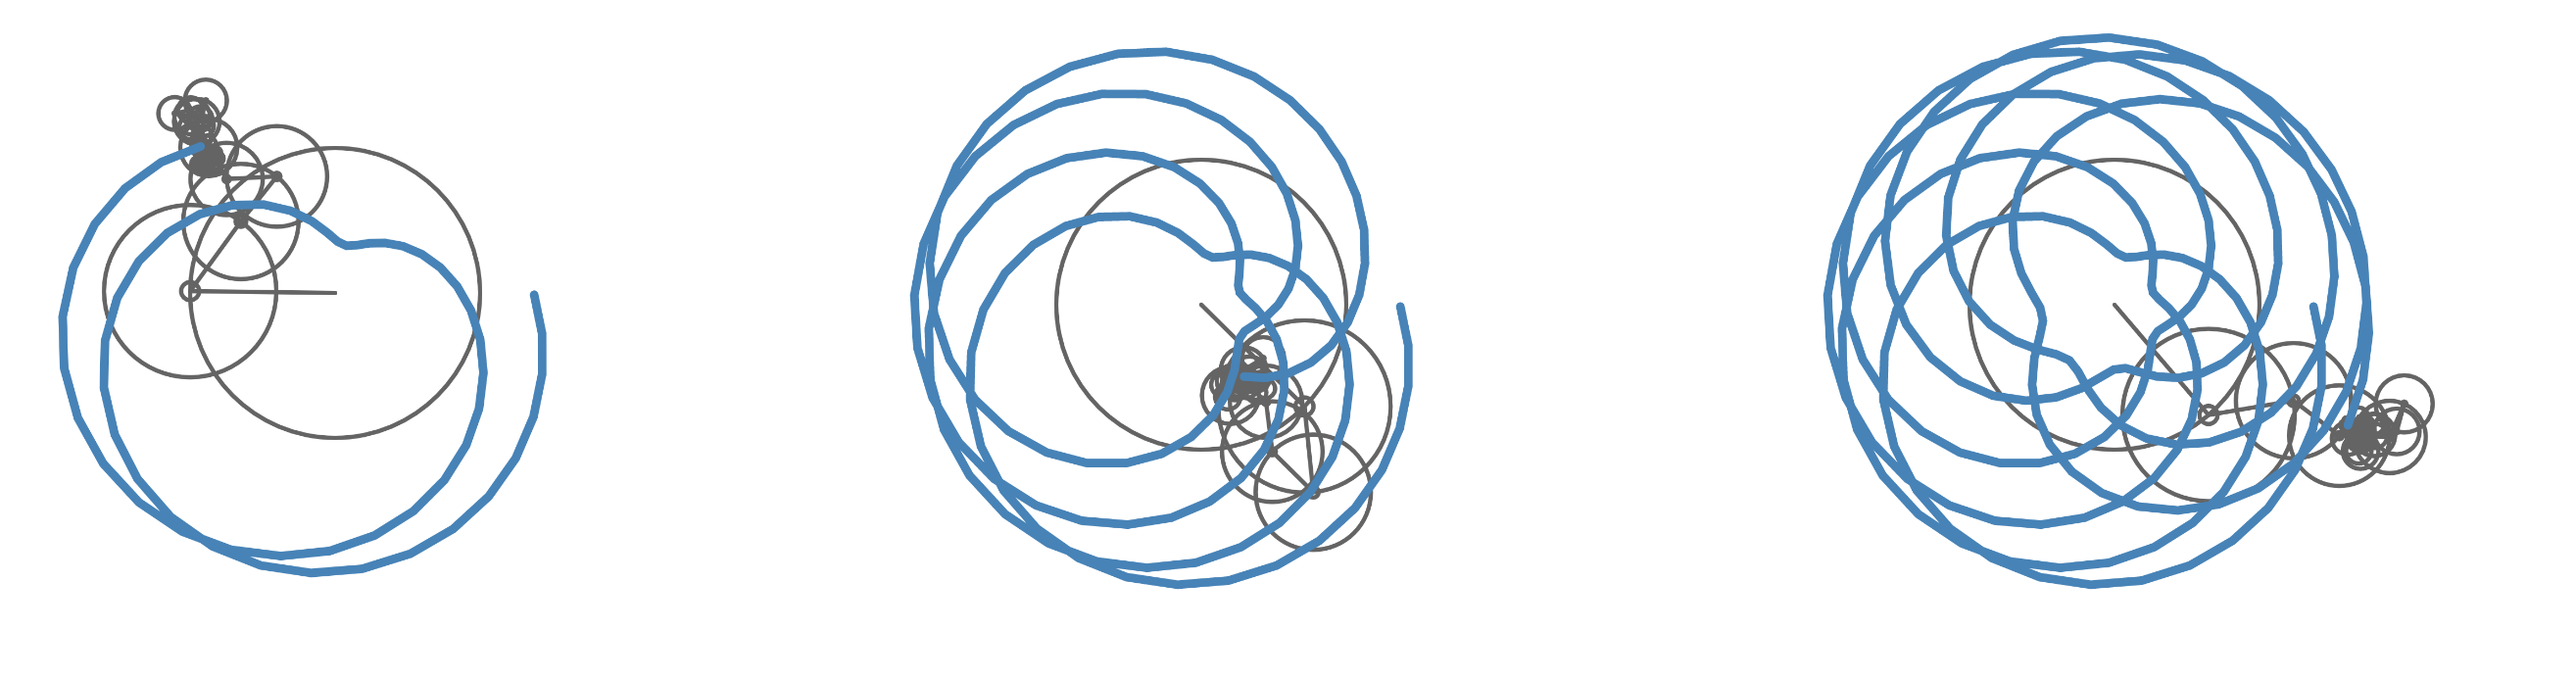
\includegraphics[width=\textwidth]{figures/marsprogressive.png}
    \caption{Caption}
    \label{fig:marsProgressive}
\end{figure}

Do we really need 365 epicycles to approximate the orbit of Mars when Ptolemy's model only required 2 or 3? We can assess this by graphing the magnitude versus frequency of our Fourier Transformed points. 

From the graph shown below, there are three visible peaks.  The rest of the frequencies have very low magnitudes and thus low importance. Therefore, this plot is telling us that only three epicycles are contributing to most of the function. 

\begin{figure}
    \centering
    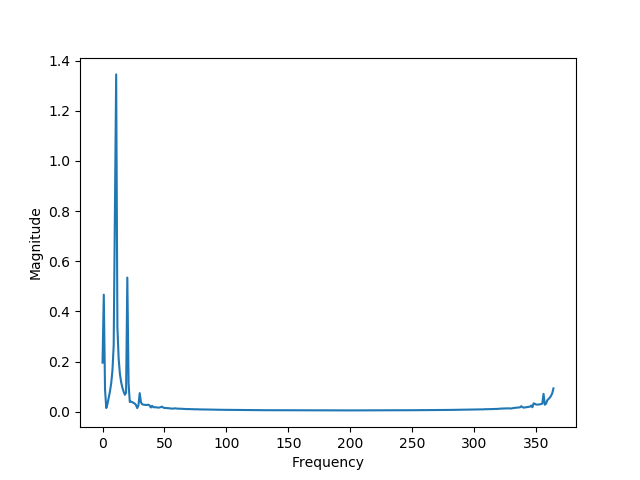
\includegraphics{figures/mars_fft.png}
    \caption{Fourier Transform plot of Mars geocentric Mars orbit}
    \label{fig:my_label}
\end{figure}

The Discrete Fourier Transform can be applied on a list of points with x and y coordinates. The resultant

The Fourier Transform has extremely powerful applications in the real world. ....
